\documentclass[paper=a4,fontsize=12pt]{scrartcl}
\usepackage[utf8]{inputenc}
\usepackage[english]{babel}
\usepackage{multirow}
\usepackage{setspace}
\usepackage[babel, german=quotes]{csquotes}
%\usepackage{hyperref}
\usepackage[style=authoryear, natbib, backend=biber]{biblatex}
\usepackage[margin = 3cm]{geometry}
\usepackage{graphicx, fancyhdr, array, wrapfig, colortbl, algorithm, algpseudocode}
%\floatname{algorithm}{Algorithmus}
%\renewcommand{\listalgorithmname}{List of algorithms}
%\renewcommand{\algorithmicend}{\textbf{Ende}}
%\renewcommand{\algorithmicif}{\textbf{Falls}}
%\renewcommand{\algorithmicthen}{\textbf{dann}}
%\renewcommand{\algorithmicelse}{\textbf{Sonst}}
%\renewcommand{\algorithmicdo}{\textbf{}}
%\renewcommand{\algorithmicwhile}{\textbf{Solange}}
%\renewcommand{\algorithmicreturn}{\textbf{Returniere}}
\renewcommand\familydefault{\sfdefault}
\linespread{1.5}
\setlength{\parindent}{4mm}
\setlength{\parskip}{2mm}
\pagestyle{fancy}
\fancyhf{}
\clubpenalty = 10000
\widowpenalty = 10000
\displaywidowpenalty = 10000
\fancyfoot{}
\rfoot{{\footnotesize \textnormal{\thepage}}}
\chead{{\footnotesize \textnormal{Variable Neighborhood Search for the Partition Graph Coloring Problem}}}
\cfoot{{\footnotesize \textnormal{Lorenz Leutgeb, Moritz Wanzenböck}}}
\lhead{{\footnotesize \textnormal{}}}
\lfoot{{\footnotesize \textnormal{\the\year}}}
\addbibresource{../pcp.bib}
\let\origappendix\appendix
\renewcommand\appendix{\clearpage\pagenumbering{roman}\origappendix}
\begin{document}
% Ein SCIENCE–Projekt ist nicht unbedingt produktorientiert, soll jedoch über eine reine Zusammenstellung von Literatur hinausgehen. Es wird eine wissenschaftlich fundierte Abhandlung und/oder Problemlösung in methodisch sauberer und nachvollziehbarer Ausarbeitung erwartet.
%foobar \cite{Lu2010, Palladino2011, Noronha2006, Li2000, Frota2010, Demange, pcp-instance-page}
\begin{titlepage}
\begin{center}
\vspace*{\fill}
{\Large P}\ {\large R\ O\ J\ E\ C\ T\ R\ E\ P\ O\ R\ T}

\vspace{5mm}

for the 

\vspace{5mm}

{\Large\bfseries Jugend Innovativ Competition 2013}

\vspace{5mm}


\includegraphics[width=10cm]{jugendinnovativ.png}

\vspace{5mm}

on the topic of 

\vspace{5mm}

{\Huge Variable Neighborhood Search for the Partition Graph Coloring Problem}

\vspace{1mm}

(J130193)

\vspace{5mm}

from

\vspace{5mm}

\begin{tabular}{>{\raggedright\arraybackslash}p{.3\textwidth}c>{\raggedleft\arraybackslash}p{.3\textwidth}}
{\large Lorenz Leutgeb} & and & {\large Moritz Wanzenböck} \\
\end{tabular}

\vspace{5mm}

under supervision from

\vspace{5mm}

{\large Dipl.-Ing.\ Dr.\ techn.\ Martin Gruber}

\vspace{5mm}

at

\vspace{5mm}


\includegraphics[width=5cm]{../img/htl.png}

\vspace*{\fill}
\end{center}
\end{titlepage}
\tableofcontents
\newpage

% Wie entstand die Projektidee?
% Was ist das Ziel der Projektarbeit?
% Welche Recherchen wurden getätigt?
%- Wie wurde der Projektablauf terminlich festgelegt (Meilensteine)?
% Wie war die Aufgabenverteilung und Ressourcenplanung? (Kooperationen mit außerschulischen Partnern)
\section{Basic idea and concept}
%\section{Projektentstehung und -planung}

Providers of internet infrastructure face the problem of satisfying an ever growing need to communicate. There are two main approaches to this problem. Providers can either expand their current network by adding additional devices or they can use their current infrastructure more efficiently.

%Betreiber der Internetinfrastruktur stehen vor dem Problem, immer weiter steigende Kommunikationsbedürfnisse befriedigen zu müssen. Dafür müssen entweder die bestehenden Netze effizienter genutzt, oder die Infrastruktur erweitert werden.

In a modern fiber-optic network, which uses Wavelength Division Multiplexing, the number of different wavelengths used to communicate directly corresponds to the efficiency of the network. The fewer wavelengths are used, the better. By optimizing the assignment of wavelengths a network can transfer more data without the need of additional hardware. This leads to an overall cheaper network without a drop in performance.

%Innerhalb von Glasfasernetzwerken, die Wavelength Division Multiplexing einsetzen, soll die Anzahl verschiedener Lichtfarben beziehungsweise Wellenlängen verringert, also optimiert werden. Dadurch können vorhandene Ressourcen besser ausgelastet und die Anschaffung und der Betrieb neuer Infrastruktur zumindest hinausgezögert werden, wodurch sich sowohl Anschaffungs- als auch Betriebskosten einsparen lassen.

The minimization of the number of used wavelengths is not a trivial problem though. It is in fact an NP-hard optimization problem. A partitioned graph is created to represent the fiber-optic network, hence the name
Partition Graph Coloring Problem. Only a selected few approaches to this problem have been published so far.

%Die Anzahl der Wellenlängen in einem solchen Netzwerk zu minimieren ist nicht trivial, es handelt sich um ein NP-schwieriges Optimierungsproblem. Modelliert werden die Glasfasernetze in Form von partitionierten Graphen. In der einschlägigen Literatur sind nur einige, wenige Lösungsansätze für dieses Problem bekannt. 

Over the course of this project we intend to implement and test a number of new approaches. These new approaches are all inspired by already existing technology. Our goal is to create a computer program which 
yields better results than the existing approaches. 

%Im Rahmen dieses Projektes sollen neuartige Wege zur Lösung des Problems implementiert und getestet werden. Ausgehend von bestehenden Technologien sowie bereits erprobten Lösungsansätzen, soll ein Programm entstehen, welches bessere Ergebnisse liefert als seine bereits bekannten Konkurrenten.

The idea to work on this project developed after a lengthly discussion with Univ-Prof.~Dipl.-Ing.~Dr.techn.~Günther~Raidl (Vienna University of Technology, Algorithms and Data Structures Group). He proposed a number of different optimization problems for our diploma thesis and still gives us feedback and support.

%Die Projektidee entstand nach ausführlicher Beratschlagung und Diskussion mit Univ-Prof.~Dipl.-Ing.~Dr.techn.~Günther~Raidl (Technische Universität Wien, Arbeitsbereich für Algorithmen und Datenstrukturen), welcher mehrere Probleme aus dem Bereich der Optimierung als Diplomarbeit vorschlug. Auch wird die Arbeit weiterhin von ihm unterstützt, sollte es Fragen zur Problemstellung oder konkreten Lösungsansätzen geben.

Our goal is to develop a new algorithm which can compete with already existing techniques. To facilitate the comparison between this new method and the old ones, a program will be implemented which is then used to solve instances of the problem. These instances originate from technical literature and hence any results can be easily compared.

%Ziel ist es, einen neuen Algorithmus zu entwickeln, welcher mit bestehenden Lösungs\-an\-sätz\-en konkurrieren kann. Zu diesem Zwecke wird der Algorithmus in ein konkretes Programm implementiert, um ihn auf die in der Literatur verwendeten Probleminstanzen anzuwenden.

Apart from technical literature, which we are provided with by Vienna University of Technology we also checked different code libraries and revision control software. Different code libraries were tested until a suitable one was found. To efficiently test and run our newly developed program, we were allowed to use the computing cluster of Vienna University of Technology.

%Neben der fachspezifischen Literatur, welche von der Technischen Universität Wien zur Verfügung gestellt wurde, befassten wir uns zu Beginn des Projekts auch mit der Recherche für geeignete Codebibliotheken und verteilte Versionskontrollsysteme. Weiters wurde die Benutzung des Computing Clusters der Universität ermöglicht, um Berechnungen schneller durchführen zu können.

\section{Solving the Partition Graph Coloring Problem}

\subsection{Problem}
In technical publications the problem is known as Partition Graph Coloring Problem (PCP). PCP is an optimization problem in the realm of network design or rather in the realm of planning the communication in an all-fiber-optic network. In most fiber-optic networks Wavelength Division Multiplexing (WDM) is used to transmit two or more communication channels over the same optic fiber. This is possible by using different wavelengths for each channel, as long as these wavelengths are sufficiently destinguishable. To minimize the complexity of a single switch within the network a single communication channel uses only one wavelength on its way through the network.

%Bei der in der Literatur als Partition Graph Coloring Problem bezeichneten Aufgabenstellung handelt es sich um ein Optimierungsproblem aus dem Bereich des Netzwerkdesigns, konkret um die Planung der Kommunikation in Glasfasernetzwerken. In diesen Netzen wird Wavelength Division Multiplexing betrieben, welches es ermöglicht, zwei oder mehr Übertragungskanäle über die selbe Glasfaser zu leiten, wenn jeder Kanal eine andere Wellenlänge verwendet und somit die anderen Übertragungen nicht stört. Um die Komplexität in einzelnen Netzwerkknoten gering zu halten wird davon ausgegangen, dass eine Verbindung von der Quelle bis zum Ziel nur genau eine Wellenlänge nutzt und diese nicht an Knotenpunkten verändert werden kann.

By using WDM different communications can be simultaneously transmitted over one fiber, as long as two different wavelengths are used. However, the maximum number of possible wavelengths per fiber is limited. If the number of used wavelengths can be minimized for all communications that are known in advance (the communication between two internet service providers can for instance be seen as a constant need to communicate, unless there are no unexpected network failures) the network is far more efficient. By decreasing the number of predetermined wavelengths a network is able to handle a higher number of spontaneous communications. In addition, an optimized network can handle more traffic and transmit the same amount of data consuming less energy. Moreover, the network can handle considerably more data before it has to be expanded.

%Zwei unterschiedliche Verbindungen können also nur dann über die selbe Netzwerkstrecke transportiert werden, wenn sie verschiedene Wellenlängen verwenden. Weiters ist die maximale Anzahl an möglichen Wellenlängen pro Strecke beschränkt. Minimiert man in diesem Szenario die Anzahl an benötigten Wellenlängen für die gesamten vorab bekannten Kommunikationsbedürfnisse (z.B.\ im großen Maßstab der Datenaustausch zwischen verschiedenen Providern, deren Verbindungen -- solange es zu keinen Ausfällen kommt -- über eine gewisse Zeit als konstant angesehen werden können), schafft man damit Platz für zusätzliche Datentransfers. Damit kann die bestehende Infrastruktur besser ausgenutzt werden, womit Kosten und Energie für den Ausbau und den Betrieb neuer Netzteile eingespart werden können.

This problem is a generalization of the Graph Coloring Problem (GC), which is well known in combinatorial optimization. Instead of coloring a single vertex, clusters of nodes must be taken into account: for each communication that is known in advance, a selection of possible routes through the network is computed (for example based on the routes length or bandwidth). Each communication represents a cluster of different vertices and each vertex represents a different route through the network. In the resulting graph -- also referred to as conflict graph -- every vertex has an edge to another vertex when the routes they represent share the same optic fiber somewhere in the network. These edges indicate that these two vertices must not share the same color, as this would result in an error while communicating (see figure \ref{fig:translation}). To solve the problem, one representative vertex has to be selected for each cluster (and by that selecting a route through the network for each communication). Additionally all selected vertices must be colored in such a way, that no two vertices that are connected by the same edge use the same color (the color represents the wavelength used for a communciation). By simultaneously trying to minimize the use of different colors (which leads to fewer used wavelenghts, thereby making room for additional network traffic) this can be expressed as  an optimization problem. This problem is known as Partition Graph Coloring Problem and is known to be NP-hard.

%Dese Aufgabenstellung kann auf einfache Art und Weise in ein generalisiertes Graph Coloring Problem transformiert werden, bei dem statt einfacher Knoten ganze Cluster von Knoten betrachtet werden müssen: Für jede Kommunikation werden vorab mehrere günstige Wege durch das Netzwerk von der Quelle zum Ziel ausgewählt (z.B.\ auf Basis der Weglänge und/oder der Übertragungsgeschwindigkeit). Jede Kommunikation bildet dabei einen eigenen Cluster, die einzelnen vorselektierten Wege dieser Kommunikation die Knoten innerhalb des Clusters. In diesem Graphen -- in der Folge auch \emph{Konfliktgraph} genannt -- werden zwei Knoten dann miteinander verbunden, wenn die jeweiligen Wege im originalen Glasfasernetzwerk eine gemeinsame Übertragunsstrecke besitzen, sie sich also gegenseitig stören würden, wenn sie die gleiche Wellenlänge verwenden würden (siehe auch Grafik \ref{fig:translation}). Ziel ist es nun, in diesem Graphen für jeden Cluster genau einen Knoten auszuwählen (für eine Kommunikation einen Weg durch das Netzwerk festlegen) und die pro Cluster ausgewählten Knoten so einzufärben, dass keine direkt miteinander verbundenen Knoten die selbe Farbe erhalten (die Farbe entspricht dabei der Zuordnung einer Wellenlänge). Minimiert man hierbei gleichzeitig die Anzahl an benötigten Farben (womit die Grundauslastung des Netzwerks reduziert wird), erhält man das generalisierte (oder auch Partition) Graph Coloring Problem, ein NP-schweres Optimierungsproblem.

\begin{figure}
    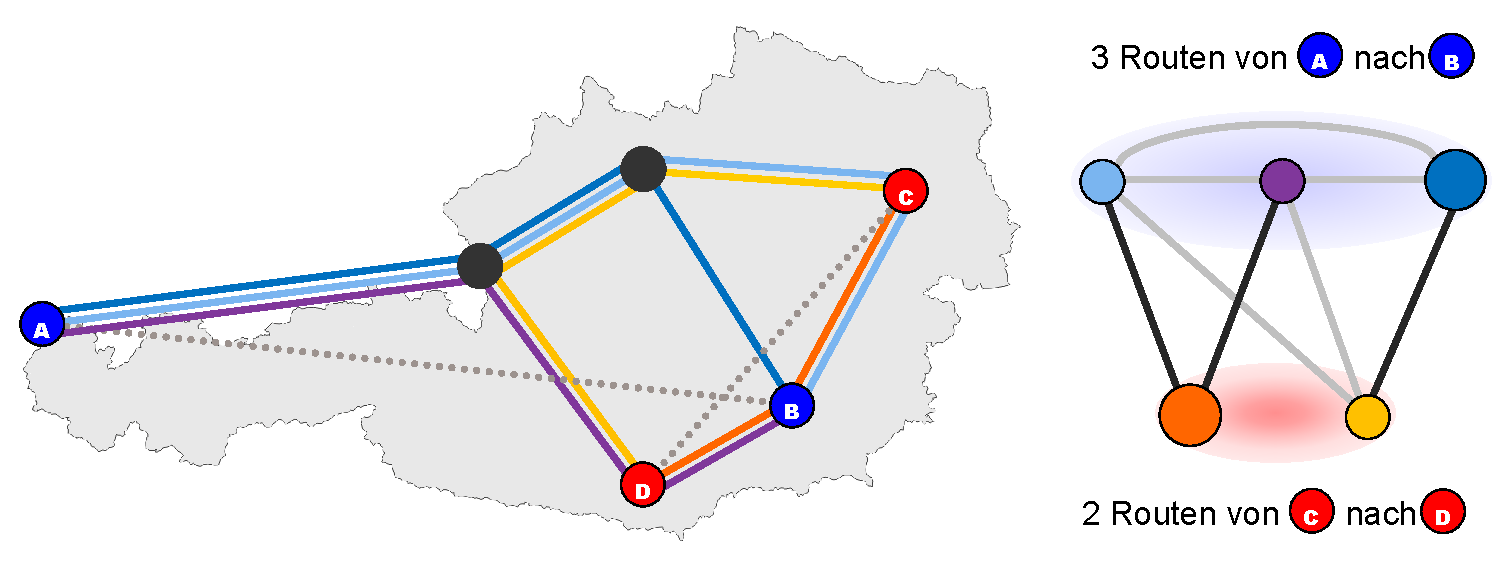
\includegraphics[width=1.0\textwidth]{../img/translation.pdf}
    \caption[Simplified test instance]{Simplified test instance: Three different routes were chosen for the communication between \emph{A} and \emph{B} (blue colors). Only two different routes were chosen for the communication between \emph{C} and \emph{D} (yellow/orange). The resulting conflict graph on the right has two clusters, each representing one communication. The edges between two vertices indicate a shared optical fiber along the routes they represent. By choosing the vertices that are indicated by bigger nodes in their respective cluster, a solution that requires only one color can be found. This means that all communications in this network can be handled with only one wavelength.}
%    \caption[Simplifizierte Testinstanz]{Simplifizierte Testinstanz: Für die Kommunikation zwischen \emph{A} und \emph{B} wurden drei mögliche Wege ausgewählt (in Blautönen gehalten), zwischen \emph{C} und \emph{D} zwei Wege (Gelb/Orange). Der daraus resultierende Konfliktgraph auf der rechten Seite enthält zwei Cluster mit drei bzw.\ zwei Knoten und die jeweiligen Kanten, wenn zwei Kommunikationswege zumindest eine Strecke im Netzwerk gemeinsam verwenden. Wählt man die größer dargestellten Knoten innerhalb der Cluster, so kann der Konfliktgraph mit nur einer Farbe gefärbt werden, d.h.\ die Kommunikationsbedürfnisse in diesem Netzwerk können mit nur einer Wellenlänge abgewickelt werden.}
    \label{fig:translation}
\end{figure}

In technical literature there is an array of different exact algorithms which reliably deliver the best solution to any given instance. However, because of the complexity of the problem, these exact algorithms can only be applied to very small instances. There are also a few heuristical approaches and algorithms which can compute solutions, however without the certainty of a proven best solution.

%In der Literatur werden exakte Algorithmen beschrieben, die beweisbar optimale Lös\-ung\-en erzeugen, aber aufgrund der Komplexität des Problems nur auf relativ kleine Netzwerke angewendet werden können. Weiters existieren einfache Konstruktionsheuristiken für die schnelle Generierung gültiger Ausgangslösungen sowie ein Ansatz mittels Tabu-Suche, der gute Ergebnisse für größere Netzwerke liefert.

\subsection{Solving the Partition Graph Coloring Problem}

%\subsection{Verfahren zur Lösung des generalisierten Graph Coloring Problems}

In the following section we will discuss already existing approaches to solving the Partition Graph Coloring Problem. Additionally we will present our own approach which facilitates already known and tested techniques in optimization problems.

%Im Folgenden sollen bereits bestehende Lösungsansätze für das Partition Graph Coloring Problem vorgestellt und kurz behandelt werden. Außerdem wollen wir unseren eigenen Lösungsansatz vorstellen, welcher auf bereits bestehenden Techniken fußt.

\subsubsection{Existing approaches}

%\subsubsection{Bestehende Lösungsansätze}

In the course of our research, we discovered a few already existing approaches to the relatively new Partition Graph Coloring Problem. \citet*{Li2000} suggested a variety of construction heuristics, which were also used by \citet*{Noronha2006} to implement their Tabu Search. Moreover, \citet*{Lu2010} proposed a different kind of algorithm which lead to \citet*{Palladino2011} suggesting a new Branch-and-Cut algorithm.

%Bei unserer Recherche fanden wir bereits einige vorhandene Lösungsansätze für das relativ junge Partition Graph Coloring Problem. \citet*{Li2000} schlugen mehrere Konstruktionsheuristiken vor, welche auch von \citet*{Noronha2006} genutzt wurden, um ihre Tabu-Suche zu implementieren.
%Desweiteren gibt es einen Algorithmus von \citet*{Lu2010} sowie einen Ansatz mit Hilfe eines Branch-and-Cut Algorithmus von \citet*{Palladino2011}.

\citet*{Li2000} described multiple variants of Greedy algorithms to give an approximate solution to the problem. From these different variants the algorithm \emph{onestepCD} looked most promising:

%\citet*{Li2000} beschreiben mehrere schnelle Greedy Algorithmen zur näherungsweisen Lösung des Problems. Im Vergleich der benötigten Farben schneidet dabei der Algorithmus \emph{onestepCD} am besten ab:

\paragraph{onestepCD}{
\label{sec:construct}
Before the \emph{onestepCD} algorithm can me applied to a problem, some preprocessing needs to be done. Every edge that connects two vertices in the same cluster is removed from the graph because every communication only needs one route through the network. Hence only one vertex per cluster must be selected, which makes all edges inside a cluster obsolete. Now the algorithm determines the vertex with the least number of colored neighboring vertices in a cluster. This step is repeated for every cluster. Once the process has been completed the vertex with the overall least number of colored neighbors is selected as the next to be colored. In case of ties the vertex with the most uncolored neighbors is selected or, if there is still a tie, the first vertex in the candidate list. The freshly selected vertex is then colored with the lowest possible color, meaning the first color that does not lead to conflicts with existing colored vertices. Then all vertices of the chosen cluster except the selected one are removed from the graph and the algorithm begins anew until every cluster has exactly one representative and is colored. 

%Zunächst werden in einem Vorverarbeitungsschritt alle Kanten aus dem Konfliktgraphen entfernt, die Knoten innerhalb eines Clusters miteinander verbinden (da für jede Kommunikation nur genau ein Kommunikationsweg gewählt wird, können sich Knoten eines Clusters nie gegenseitig stören, die entsprechenden Kanten sind daher für die Lösung des Problems irrelevant und können gelöscht werden). Danach wird für jeden Cluster der Knoten mit der geringsten Anzahl an bereits eingefärbten Nachbarknoten bestimmt, der Knoten mit der insgesamt kleinsten Anzahl wird ausgewählt. Gibt es hier mehrere gleichwertige Kandidaten, wird aus diesen der Knoten mit der größten Anzahl an noch nicht eingefärbten Nachbarknoten gewählt bzw. -- falls dies immer noch nicht eindeutig möglich ist -- der erste Knoten aus diesen Kandidaten. Nachdem nun ein Knoten als Repräsentant für seinen Cluster bestimmt und ihm die kleinstmögliche Farbe zugewiesen wurde, werden alle anderen Knoten, die sich im selben Cluster befinden, gelöscht. Der Prozess wird solange fortgeführt, bis die Repräsentanten aller Cluster gewählt und eingefärbt sind.
}

This algorithm can get valid solutions extremely quickly. The downside, however, is that only in rare cases the computed solution is also the best solution, meaning the number of used colors cannot be reduced any further. On the upside the computed solution can be used as a starting point for improvement processes.

%Diese Vorgehensweise führt schnell zu einer gültigen Lösung, die aber nur in den seltensten Fällen auch wirklich optimal bezüglich der Anzahl an benötigten Farben ist. Sie kann aber als Ausgangspunkt für Verbesserungsverfahren dienen.
 
\paragraph{Tabu Search}{
\citet*{Noronha2006} described a different way to solve the PCP. Their algorithm, a Tabu Search, takes existing solutions as input and then proceeds to try improving them. The work also relies on the algorithm \emph{onestepCD} to get an initial solution.

%Mit Hilfe der von \citet*{Noronha2006} vorgeschlagenen Tabu-Suche ist es möglich, eine bereits bestehende Lösung durch verschiedene Transformationen in eine neue, nach Möglichkeit bessere Lösung zu verwandeln.

The Tabu Search begins by recoloring all vertices who use the highest color with a random, smaller color. Due to this recoloring process, some vertices come in conflict with one another. 

%Zunächst wird bei der Tabu-Suche eine ungültige Lösung erzeugt, und zwar durch das neue Färben aller Knoten, welche in der Ausgangslösung noch die höchste Farbe besaßen, mit einer zufälligen, kleineren Farbe.

These deliberately created conflicts are then stored in a list. The algorithm consequently proceeds to try and solve this conflict by selecting a random vertex and recoloring it with a random color. If this step leads to a solution with fewer conflicts, the Tabu Search marks the vertex as done and proceeds to try solving other conflicts.

%Nachdem nun natürlich Konflikte zwischen zwei verbunden Knoten mit der gleichen Farbe entstanden sind, versucht die Tabu-Suche diese Konflikte zu lösen. Dazu wird ein zufälliger im Konflikt stehender Knoten ausgewählt und es wird versucht, diesen neu einzufärben. Sollte dies Erfolg haben beginnt die Tabu-Suche wieder bei der Suche nach in Konflikt stehenden Knoten.

If, however, the algorithm cannot find a suitable color for a vertex, that same vertex is added to a tabu list where it remains for a specified amount of iterations. All vertices on the tabu list are forbidden from being recolored, effectively fixing their color for as long as they are on the tabu list.

%Sollte für einen Knoten allerdings keine passende Farbe gefunden werden können, wird dieser Knoten auf die Tabu-Liste gesetzt, wo er für einige Iterationen verbleibt. Knoten sind, solange sie auf dieser Liste sind, tabu für eine Neueinfärbung, dürfen also nicht ausgewählt werden.

When the Tabu Search reaches a state with zero conflicts, the algorithm begins anew. The solution in turn becomes the input for the Tabu Search, and all the steps described above are taken again. If, however, the Tabu Search does not find a valid solution, even after many iterations, the Tabu Search stops and returns the last known result.}

%Ist die Tabu-Suche nun nach mehreren Iterationen zu einer validen Lösung gekommen, welche weniger Farben als die Ausgangslösung verwendet, wird sie erneut aufgerufen, um nach Möglichkeit wieder ein Ergebnis mit einer Farbe weniger zu berechnen.
%Sollte hingegen die Tabu-Suche auch nach vielen Iterationen keine gültige Lösung erzeugen können, bricht sie von selbst ab und gibt ihre Verbesserungsversuche für diese Lösung auf und beginnt mit einer neuen, zufälligen Neufärbung der aktuell besten gefundenen Lösung.}

\subsubsection{Variable Neighborhood Search (VNS)}
We decided to use already tried and tested techniques in optimization as the starting point of our project. We then proceeded to adapt these techniques to the specific needs of the Partition Graph Coloring Problem.

%Als Ausgangspunkt für unser Projekt setzen wir auf bereits bewährte Techniken aus anderen Bereichen der Optimierung und versuchen, diese bestmöglich für das Partition Graph Coloring Problem einzusetzen.

\paragraph{Initial solution}{
To get a valid starting solution which can then be improved, we relied on already existing algorithms. The specific algorithm \emph{onestepCD} we used is already discussed in section~\ref{sec:construct}. It was chosen for its fast runtime while simultaneously providing good results compared to similar algorithms.

%Um eine gültige Startlösung als Ausgangspunkt der Variablen Nachbarschaftssuche zu berechnen, wird wie gemeinhin üblich eine schnelle Konstruktionsheuristik eingesetzt. Konkret wurde nach der Konsultation von \citet*{Li2000} die dort beschriebene Heuristik \emph{onestepCD} (siehe \ref{sec:construct}) gewählt.
}

% Im folgenden soll erläutert werden, wie mit diesem Algorithmus eine Lösung gefunden wird.
\paragraph{Structure of a Variable Neighborhood Search}{
The Variable Neighborhood Search is a metaheuristic that is used to solve different optimization problems. A metaheuristic is a special kind of algorithm that controls other heuristics (and in some cases also exact) methods and combines their results into an overall better solution.

%Bei der Variablen Nachbarschaftssuche handelt es sich um eine metaheuristische Methode, um verschiedenste Optimierungsprobleme zu lösen. Als Metaheuristik bezeichnet man dabei Algorithmen, die andere heuristische (und manchmal auch für Teilprobleme exakte) Optimierungsverfahren steuern und deren Ergebnisse sammeln und kombinieren.

The VNS uses different Neighborhoods, hence the name Variable Neighborhood Search. It can be used to improve already existing solutions to a problem. A Neighborhood is defined by different \emph{Moves} that are made to get from one solution to another. This new solution is ideally an improvement of the current one. Moves can be any kind of change in a solution. A single recolored vertex, for instance, can be seen as a Move. By executing a Neighborhood over and over again until no more improvement is achieved, the algorithm reaches a \emph{local optimum}. Nevertheless this local optimum in most cases is not the global one.

%Wie der Name bereits suggeriert versucht eine VNS auf Basis unterschiedlicher Nachbarschaften eine bereits bestehende, nicht optimale Lösung zu verbessern. Eine Nachbarschaft wird im Normalfall durch sogenannte \emph{Moves}, also Züge, definiert, die be\-schrei\-ben, wie man von einer Lösung zu einer Nachbarlösung kommt, die hoffentlich besser als die Ursprungslösung ist. Ein solcher Zug kann z.B.\ die Auswahl eines anderen Knotens als Repräsentant eines Clusters sein. Kann eine Lösung mit Zügen aus einer Nachbarschaft nicht mehr verbessert werden, dann befindet man sich in einem \emph{lokalen Optimum}, das leider im Normalfall nicht dem globalen Optimum -- der besten möglichen Lösung -- entspricht.

A special optimization component of the Variable Neighborhood Search is the \emph{Variable Neighborhood Descent} (VND). By using VND several different Neighborhoods are executed one after the other. This helps to further optimize a solution, because the local optimum of one Neighborhood can be very different from that of another. VND tries not to get stuck in the local optimum of one Neighborhood by executing a different one after an improvement was found. This keeps the improvement process going, even if one Neighborhood reaches its local optimum. 

%Die Variable Nachbarschaftssuche setzt nun in ihrer Optimierungskomponente (\emph{Variable Neighborhood Descent}, VND) nicht nur eine sondern gleich mehrere unterschiedliche Nachbarschaften hintereinander ein in der Hoffnung, dass ein lokales Optimum einer Nachbarschaft nicht zwangsläufig auch ein lokales Optimum einer anderen Nachbarschaft ist. Man setzt also darauf, dass eine Lösung, die in einer Nachbarschaft nicht mehr verbessert werden kann, in einer anderen Nachbarschaft sehr wohl noch Optimierungspotential besitzt. Diese neue Lösung kann dann vielleicht wieder mit einem Zug aus der ursprünglichen Nachbarschaft verbessert werden und so weiter.

The VND systematically cycles through all the different possible Neighborhoods by using the \emph{Best Improvement Strategy}, that is by using the move with the best overall performance of all possible moves. The process stops only if a local optimum for all Neighborhoods is found. This local optimum, however, can still be far from the global optimum, which means the VNS has to do some work to help the Neighborhoods to further optimize the solution.

%Durchsucht man alle definierten Nachbarschaften systematisch (z.B.\ mittels \emph{Best Improvement} Strategie, d.h.\ von allen möglichen Zügen innerhalb einer Nachbarschaft wird jener gewählt, der die Lösung maximal verbessert) hintereinander und wiederholt nach besseren Lösungen, dann stoppt dieser Prozess erst dann, wenn eine Lösung gefunden wurde, die ein lokales Optimum bezüglich sämtlicher Nachbarschaften darstellt.

\begin{figure}
\begin{center}
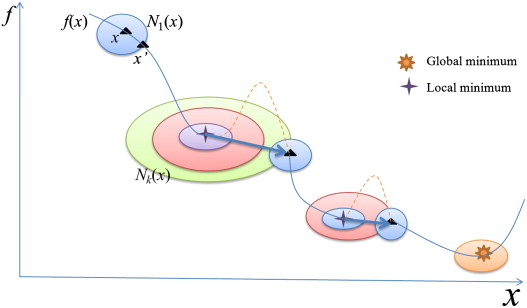
\includegraphics{../img/vns.jpg} %TODO gruber bild
\end{center}
\caption{Graphic representation of Variable Neighborhood Search. \cite{Chen}} %TODO remove cite
\end{figure}

In case the VNS gets stuck in a local optimum for all Neighborhoods it uses \emph{shaking}. By shaking a solution, that solution will be randomly altered. These changes do not necessarily lead to an improvement, they are only used to compute a new starting point for VND. If a small alteration in the globally best solution does not lead to a better result after VND, the changes grow more drastic with each unsuccessfull shake. This leads to more diverse starting positions and could potentially give better overall results.

%Um diesem Zustand des vollkommenen Stillstandes zu entkommen, wird, nachdem dieses lokale Optimum für alle definierten Nachbarschaften erreicht wurde, mit immer größer werdenden Kraft die Lösung ``geschüttelt''. Gemeint ist damit, dass die lokal optimale Lösung durch verschiedene Algorithmen verändert wird, welche nicht darauf abzielen, eine Lösung besser zu machen, sondern sie zunächst ein wenig, mit dem Fortschreiten der Optimierung aber auch möglichst stark zu verfremden, um einen neuen Startpunkt für das VND zu besitzen.

The VNS can be explained using a three-dimensional plane with every point on the plane representing a unique solution to the problem. The \enquote{height} of a point can be seen as the \enquote{quality} of the solution it represents. For our problem this means the fewer colors are used the lower the point lies. For a minimization problem valleys represent good solutions while hills stand for bad solutions. The VND algorithm proceeds into such a valley step by step. This valley is not necessarily the deepest, so by using \emph{Shaking} the algorithm steps back onto a hill and hopefully finds a different, deeper valley to restart the process. It cannot be guaranteed, however, that the global optimum is reached this way.

%Veranschaulichen kann man sich das Verfahren, wenn man sich alle gültigen Lösungen als eine große Fläche vorstellt. Je nach Güte der Lösung sind einzelne Teile dieser Fläche unterschiedlich hoch, gute Lösungen bilden Senken (wenige Farben werden für die Färbung benötigt), während schlechte Lösungen Berge bilden. Das VND tendiert nun dazu, sich in einer dieser Senken festzufahren, es wurde ein lokales Optimum bezüglich sämtlicher Nachbarschaften erreicht.

%Mit Hilfe des ``Schüttelns'' wird nun versucht, aus eben jenen Senken zu entkommen, um eine andere, hoffentlich tiefere Senke zu finden, also eine bessere Lösung. Nach diesem Schritt beginnt der Algorithmus nämlich wieder von vorne und sucht mit Hilfe der Nachbarschaften erneut ein lokales Optimum.

Although the Variable Neighborhood Search can theoretically be executed infinitely, execution is stopped after a predefined amount of time or in case the currently best solution was not improved for a while.

%Obwohl die Variable Nachbarschaftssuche in der Theorie immer weiter laufen könnte und dabei hoffentlich immer wieder neue, bessere Lösungen erreicht, wird meist eine fixe Zeit oder eine Anzahl an Iterationen bzw.\ ``Schüttelungen'' ohne Verbesserung als Abbruchkriterium gewählt.

\begin{algorithm}
\begin{algorithmic}[1]
\State Compute starting solution with \emph{onestepCD}
\While{termination condition \textbf{not} fulfilled}
\State Execute Variable Neighborhood Descent with Best Improvement Strategy:
%\State Führe Variable Neighborhood Descent mit Best Improvement Strategie durch:
\State Neighborhood $l \leftarrow 1$
\While{$l \leq $ number of neighborhoods \textbf{and} time limit not reached}
\State Execute neighborhood $n_l$
\If {solution improved \textbf{and} $l\neq 1$} 
\State  $l\leftarrow 1$  
\Else
\State  $l\leftarrow l + 1$
\EndIf
\EndWhile
\If{Got new best solution \textbf{or} $k \geq k_{\mathrm max}$}
\State $k \leftarrow k_{\mathrm start}$ 
\Else
\State $k \leftarrow k + 1$
\EndIf
\State Select random neighborhood and use it to shake solution
\EndWhile
\State\Return best solution
\end{algorithmic}
\caption{Pseudocode for Variable Neighborhood Search}
\end{algorithm}
}

\subsubsection{Neighborhoods}
\label{sec:neigh}
As mentioned above Neighborhoods are small algorithms, often heuristics, that transform one valid solution into another. The result of this transformation is hopefully a better solution than the original one. In this section we will discuss the four different Neighborhoods we used to improve solutions to the PCP. These Neighborhoods are named \emph{changeColor}, \emph{changeNode}, \emph{DSTAUR}, and \emph{changeAll}.

%Wie bereits beschrieben handelt es sich bei Nachbarschaften um einzelne Algorithmen die versuchen, eine gültige Lösung in eine andere, bessere Lösung durch eine relativ kleine Änderung umzuwandeln. Wir haben uns zunächst auf die drei Nachbarschaften \emph{changeColor}, \emph{changeNode} und \emph{DSATUR} konzentriert, wobei weitere Nachbarschaften noch zur Diskussion stehen.

Every Neighborhood also implements a unique way of \emph{shaking} a solution that makes use of the same moves as its optimization counterpart but ignores the objective function, that means not only improving moves are accepted.

%Jede Nachbarschaft bietet auch eine Methode an, eine Lösung zu ``schütteln'', welche ähnlich abläuft wie die Methode zur Suche des jeweiligen lokalen Optimums, allerdings ohne die Beschränkung ausschließlich bessere Ergebnisse zurück liefern zu müssen.

\paragraph{changeColor}
This very simple Neighborhood was inspired by the Tabu Search of \citet*{Noronha2006}. Each color is represented by a number. The Neighborhood chooses the vertices with the currently highest color and tries to recolor them.

%Bei dieser sehr einfachen Nachbarschaft, die von der Tabu-Suche aus \citet*{Noronha2006} inspiriert ist, wird versucht, alle Knoten umzufärben, welche mit der höchsten Farbe markiert wurden. 

To reach its goal, the Neighborhood first selects a vertex colored with the highest color. This vertex is then randomly recolored, even if this leads to conflicts in the solution. The algorithm then proceeds to find new suitable colors for all adjacent vertices of the selected one. 

%Um dieses Ziel zu erreichen, werden alle Knoten, welche diese höchste Farbe besitzen, mit einer neuen zufälligen Farbe markiert. Dies führt natürlich unweigerlich zu Konflikten zwischen verbundenen Knoten im Konfliktgraph, d.h.\ zu benachbarten Knoten mit gleicher Farbe. 

When a suitable color is found, that vertex is recolored. If no suitable color can be found for only a single adjacent vertex, the next lowest color is used to color the selected vertex. These steps are repeated until a suitable color combination can be found. Once this combination is found, the algorithm searches for other vertices using the highest color.

%Um diese Konflikte zu lösen wird ein zufälliger, im Konflikt stehender Knoten ausgewählt, um ihn mit einer passenden Farbe zu füllen. Zu beachten ist hierbei die Tatsache, das diese passende Farbe kleiner sein muss als die frühere höchste Farbe, da ja eine Verbesserung (eine Reduktion der Farbenanzahl um 1) erzielt werden soll.

If, however, no suitable combination can be found and the recoloring process comes to a halt, the Neighborhood returns with no improvement made. In case the Neighborhood was a success and the newly computed solution is better than the old one, the process continues until no improvement is possible anymore.

%Sollte sich keine passende Farbe finden, wird auch dieser im Konflikt stehende Knoten mit einer zufälligen Farbe neu eingefärbt, was im Normalfall zu weiteren Konflikten führt. Es wird nun versucht, diesen gesamten Vorgang so lange zu wiederholen bis keine Konflikte mehr bestehen. 

%Sollte nach einer gewissen Anzahl an Iterationen keine konfliktfreie Lösung gefunden werden, bricht \emph{ChangeColor} automatisch ab und liefert die letzte valide Lösung zurück.

\paragraph{changeNode}
Like with \emph{changeColor}, \emph{changeNode} relies on a fast algorithm to change a solution. This is done by selecting an alternative vertex of the same cluster for each vertex colored with the highest color.

%Diese Nachbarschaft baut auf der Tatsache auf, dass man aus einem Cluster nur jeweils einen Knoten auswählen muss. Dazu werden wie bei \emph{ChangeColor} alle Knoten höchster Farbe ausgewählt und umgefärbt.

Similar to \emph{changeColor}, the algorithm searches for a vertex that currently uses the highest color. This vertex is then replaced by a different vertex from the same cluster. Then an attempt is made to recolor the replacement. If the new suitable color is less than the highest color, the replacement becomes the new selected vertex in the solution for this cluster. 

%Nun wird wieder ein zufälliger Knoten aus den entstandenen Konflikten ausgewählt, welcher dann aber durch einen zufälligen Knoten aus dem selben Cluster ersetzt wird. An diesem Knoten wird dann ein neuer Einfärbeversuch unternommen, wobei die maximal zulässige Farbe natürlich wieder kleiner ist als die ursprünglich höchste Farbe.

If no suitable color can be found and all other vertices of the cluster have been tried out without success, the Neighborhood stops. When all vertices of highest color have been replaced, a new better solution has been found.

%Dieser Vorgang wird solange wiederholt bis alle Konflikte gelöst wurden oder zu viele Iterationen abgelaufen sind.

\paragraph{NewVertexColoring-DSATUR}
This Neighborhood reduces the PCP to a normal Graph Coloring Problem without clusters. This is done by essentially fixing the current selection of vertices of all clusters. The resulting graph is colored using a greedy algorithm to solve the resulting Graph Coloring Problem which is still NP-hard. This algorithm uses the following steps to recolor the graph:

%Diese Nachbarschaft reduziert das Graph Partition Coloring Problem auf das normale Graph Coloring Problem ohne Clustering der Knoten, indem die aktuell gewählten Repräsentanten fixiert werden und dieses so vereinfachte Problem (das allerdings immer noch NP-hart ist) wird nun mit folgendem Greedy Ansatz näherungsweise gelöst:

\begin{enumerate}
	 \item Find the (still uncolored) vertex with the highest number of colored neighbors.
%    \item Finde den (noch nicht eingefärbten) Repräsentanten mit der größten Anzahl an eingefärbten Nachbarn (engl.\ Degree SATURation).
	 \item In case of a tie: Select the vertex with the highest number of uncolored neighbors.
%    \item Bei Gleichstand: Wähle den Knoten mit der größten Anzahl an nicht eingefärbten Nachbarn.
	 \item If there is still a tie: Select the first vertex in numerical order.
%    \item Bei Gleichstand wähle den ersten Knoten in lexikographischer Abfolge.
	 \item Assign the lowest possible color to the vertex.
%    \item Weise dem gewählten Knoten die kleinste mögliche Farbe zu.
	 \item Repeat this procedure until all vertices have been colored.
%    \item Wiederhole, bis die Repräsentanten aller Cluster eingefärbt wurden.
\end{enumerate}

\paragraph{changeAll}
The \emph{changeAll} Neighborhood can be seen as a combination of \emph{changeColor} and \emph{changeNode}. It simultaneously replaces a vertex of a cluster and recolors it.

First the algorithm searches for vertices of the highest color. It then replaces the found vertex with another one from the same cluster. This replacement is then recolored, much like in the \emph{changeColor} Neighborhood. 

If no suitable pair of color and replacement vertex can be found, the Neighborhood stops. When all vertices of the highest color have been replaced and recolored a better solution has been found. 

\subsubsection{Implementation}
%\subsubsection{Implementierung}
To verify and evaluate our approach, we successfully implemented the Variable Neighborhood Search as presented above with an initial solution computed by \emph{onestepCD}. 

The actual development was done using C++. C++ was chosen as it is both a very versatile and fast programming language and because many code libraries for optimization are written using C++.

%Um die im Zuge dieser Arbeit entwickelten Lösungsansätze verifizieren und bewerten zu können, wurde das vorgestellte Konzept (Variable Nachbarschaftssuche mit Ermittlung einer Initiallösung durch \emph{onestepCD}) vollständig implementiert.

%Das Programm wurde in C++ entwickelt, da diese Sprache für gute Performance bekannt ist und außerdem etablierte Codebibliotheken, speziell für Probleme der Kombinatorik und Graphentheorie, explizit für C++ zur Verfügung stehen.

After some research we decided to use the C++ code library Boost\footnote{see \url{http://www.boost.org/}}. Boost offers a vast variety of different data structures and helper functions. All of these features have been heavily tested and are easy to use, which enables a rapid programming style.

%Nach einigen Recherchen fiel die Wahl auf die Bibliothek Boost\footnote{siehe \url{http://www.boost.org/}}. Bei Boost handelt es sich um eine robuste, gut getestete und vielseitige Bibliothek, welche ein schnelles und einfaches Arbeiten ermöglicht.

Every Neighborhood discussed in section~\ref{sec:neigh} was implemented. Special attention was given to an efficient implementation of each Neighborhood, as it is essential for the overall running time.

%Alle im Abschnitt \ref{sec:neigh} besprochenen Nachbarschaften wurden umgesetzt, wobei in diesen Codeteilen auf eine effiziente Umsetzung ganz besonders geachtet wurde, da sie das Laufzeitverhalten stark prägen.

\subsection{Conclusion}
There is an increasing demand for communication in huge fiber optic networks like the ones operated by internet service providers.

%In großen Glasfasernetze, wie sie zum Beispiel von großen Internetinfrastrukturbetreibern betrieben werden, besteht ein immer größer werdendes Kommunikationsbedürfnis.

To accommodate with these ever rising demands two steps can be taken: The easier -- but also more expensive -- route is to expand existing networks by using new infrastructure. The harder -- but also cheaper -- route is to use existing networks more efficiently. The task to assign different wavelengths to a fiber optic network to enable parallel communication between many different parties can be seen as a practical application of the Partition Graph Coloring Problem. 

%Um diesen steigenden Anforderungen gerecht zu werden kann natürlich einfach die Infrastruktur -- mit entsprechenden (auch laufenden) Kosten -- erweitert werden oder aber die bestehenden Netze werden effizienter genutzt. Das Problem, mehrere Kommunikationskanäle über das selbe Glasfasernetzwerk ohne gegenseitige Störungen zu übertragen, kann allgemein auf das Partition Graph Coloring Problem zurückgeführt werden.

In this paper we introduced a new approach to solving the Partition Graph Coloring Problem by using Variable Neighborhood Search, which facilitates 4 different Neighborhoods to improve an existing solution step-by-step.

%In dieser Arbeit stellten wir eine Variable Nachbarschaftssuche vor, die mithilfe eines VND auf Basis von drei Nachbarschaften eine Ausgangslösung schrittweise verfeinert.

Initial computations of small instances showed promising results. Later tests on large instances of the given problem showed a 15\% improvement comapred to the initial solution computed by the construction heuristic. Our approach already gives good results, but we have ideas in mind to further enhance the VNS.

%Erste Tests auf kleineren Instanzen des Problems zeigten bereits vielversprechende Ergebnisse. Für größere Instanzen ist ungleich mehr Rechenzeit und -leistung notwendig, entsprechende Testläufe, um diesen Ansatz auch z.B.\ mit der Tabu-Suche von \citet*{Noronha2006} vergleichen zu können, sind erst in Vorbereitung. Um zukünftig noch bessere Ergebnisse zu erzielen wird auch die Verwendung  weiterer, problemspezifischer, allerdings auch umfangreicherer Nachbarschaften in Erwägung gezogen.

%\subsection{Innovationsgehalt des bearbeiteten Lösungsansatzes}
%\subsection{Testläufe}
%\subsubsection{Inkrementeller Entwicklungszyklus}
%\subsection{Vorschau}

% Welche Idee/Innovation steckt im Projekt?
% Welche Lösungswege wurden ins Auge gefasst?
% Welche Experimente/Versuche/Studien wurden angestellt?
% Welche Forschungsmethoden wurden angewendet bzw. entwickelt (z.B. bei Datenerhebung mittels Fragebogen oder ähnl.)?
% Wurden Interessensgruppen involviert bzw. wie wurden diese informiert (Wissenstransfer)?
% Welche Ergebnisse wurden (bisher) erzielt?
% Sollte das Projekt noch nicht abgeschlossen sein, sind die vorläufigen Ergebnisse bis dato zu dokumentieren und eine Vorschau auf das weitere Vorhaben zu erstellen.
% Wie wurde kontrolliert, ob das Ziel (bisher) erreicht wurde?
% Welcher Arbeitsaufwand steckte im Projekt?
% Welche Schlussfolgerungen sind (bis dato) daraus zu ziehen?
% Bei Sonderpreis-Projekten ist u.a. die Relevanz der ökologischen, sozialen und ökonomischen Nachhaltigkeit bzw. die wirtschaftliche Machbarkeit anzuführen.
%\subsection{Ökonomische Grundlage und ökologischer Vorteil}

\newpage
\printbibliography
\addcontentsline{toc}{section}{Literature}
\listoffigures
\addcontentsline{toc}{section}{List of figures}
\listoftables
\addcontentsline{toc}{section}{List of tables}
\listofalgorithms
\addcontentsline{toc}{section}{List of algorithms}

%Anhang: Skizzen, Grafiken, Zeichnungen, Schaltpläne, Fotos, Links zu Videos oder Websites etc.

\appendix

\section{Appendix}

\subsection{Results}

At the end of this project, we were allowed to use the computing grid of the Algorithms and Data Structures Group of Vienna University of Technology to test our program. All test instances have been taken from \cite{Noronha2006}. Each instance of the program was started with a time limit of 600s and a limit of 5000 unsuccessfull shaking runs. The results of the tests can be found in table~\ref{tab:result}.

%Mit Ende der Arbeit an dem Projekt im Rahmen der Diplomarbeit wurden in Tabelle~\ref{tab:result} ersichtliche Ergebnisse auf dem Berechnungsnetzwerk der Arbeitsgruppe für Algorithmen und Datenstrukturen des Instituts für Computergraphik und Algorithmen an der Technischen Universität Wien erzielt.

%Die Instanzen stammen von der genannten Arbeitsgruppe und sind mit jenen von \cite{Noronha2006} vergleichbar.

%Das Abbruchkriterium der VNS für diese Ergebnisse war ein Zeitlimit von 600s oder 5000 fehlgeschlagene \enquote{Schüttelversuche}.


\subsubsection*{Description}

\begin{description}
    \item[Instance] Name of the computed instance.
    \item[$|V|$] Number of vertices in that instance.
    \item[$|E|$] Number of edges in that instance.
    \item[$|C|$] Number of clusters in that instance.
    \item[$S_i$] Number of colors used by the construction heuristic \emph{onestepCD}.
    \item[$N$] Used Neighborhoods in order of iteration:
        \begin{description}
            \item[\texttt{c}] \emph{ChangeColor}
            \item[\texttt{n}] \emph{ChangeNode}
            \item[\texttt{a}] \emph{ChangeAll}
            \item[\texttt{d}] \emph{DSATUR}
        \end{description}
    \item[$S_{avg}$] The average number of colors used by our program. Every test instance was run 40 times to avoid statistical anomalies.
    \item[$S_{\sigma}$] The mean deviation of our results. Due to randomization happening in each of the 40 runs anomlies may occur.
    \item[$S_{\Delta}$] Relative improvement when compared to the construction heuristic.
    \item[$t$] Average runtime in seconds.
\end{description}

\singlespacing
\begin{table}[p]
\centering
\begin{tabular}{|c|ccc|c|c|ccc|c|c|}
\hline
Instance & \multicolumn{1}{c}{$|V|$} & \multicolumn{1}{c}{$|E|$} & \multicolumn{1}{c|}{$|C|$} & \multicolumn{1}{c|}{$S_i$} & \multicolumn{1}{c|}{$N$} & $S_{min}$ & \multicolumn{1}{c}{$S_{avg}$} & \multicolumn{1}{c|}{$S_{\sigma}$} & \multicolumn{1}{c|}{$S_{\Delta}$} & \multicolumn{1}{c|}{$t$} \\
\hline\hline

\multirow{3}{*}{\texttt{dsjc500.5-1.in}} & \multirow{3}{*}{500} & \multirow{3}{*}{62624} & \multirow{3}{*}{500} & \multirow{32}{*}{69} &
      \texttt{cnad}	& \multirow{3}{*}{62}	& 63.67	& 0.52	& \multirow{3}{*}{11.29}	& 494109.3\\
&&&&& \texttt{cand}	&			& 63.55	& 0.55	&				& 494685.3\\
&&&&& \texttt{acnd}	&			& 63.67	& 0.52	&				& 492537.0\\
\cline{1-4}\cline{6-11}
\multirow{14}{*}{\texttt{dsjc500.5-2.in}} & \multirow{14}{*}{1000} & \multirow{14}{*}{249671} & \multirow{14}{*}{500} & &
      \texttt{cnda}	& \multirow{14}{*}{60}	& 61.30	& 0.51	& \multirow{14}{*}{15.00}	& 482239.0\\
&&&&& \texttt{cadn}	&			& 61.27	& 0.50	&				& 472219.3\\
&&&&& \texttt{dcan}	&			& 61.55	& 0.55	&				& 488494.5\\
&&&&& \texttt{danc}	&			& 61.40	& 0.54	&				& 497711.0\\
&&&&& \texttt{ncda}	&			& 61.13	& 0.40	&				& 496069.8\\
&&&&& \texttt{ndca}	&			& 61.27	& 0.50	&				& 499308.0\\
&&&&& \texttt{ndac}	&			& 61.17	& 0.49	&				& 508483.5\\
&&&&& \texttt{nacd}	&			& 61.45	& 0.55	&				& 448795.8\\
&&&&& \texttt{nadc}	&			& 60.95	& 0.31	&				& 499959.3\\
&&&&& \texttt{acdn}	&			& 60.88	& 0.40	&				& 489919.3\\
&&&&& \texttt{adcn}	&			& 60.80	& 0.40	&				& 502662.8\\
&&&&& \texttt{adnc}	&			& 60.95	& 0.31	&				& 509733.8\\
&&&&& \texttt{ancd}	&			& 61.70	& 0.51	&				& 443322.5\\
&&&&& \texttt{andc}	&			& 61.00	& 0.45	&				& 499170.8\\
\cline{1-4}\cline{6-11}
\multirow{14}{*}{\texttt{dsjc500.5-3.in}} & \multirow{14}{*}{1500} & \multirow{14}{*}{562401} & \multirow{14}{*}{500} & &
      \texttt{cdna}	& \multirow{14}{*}{60}	& 61.20	& 0.46	& \multirow{14}{*}{15.00}	& 477578.0\\
&&&&& \texttt{cadn}	&			& 61.20	& 0.51	&				& 465780.5\\
&&&&& \texttt{dcna}	&			& 61.38	& 0.53	&				& 479848.8\\
&&&&& \texttt{dnac}	&			& 61.23	& 0.52	&				& 498028.5\\
&&&&& \texttt{danc}	&			& 61.23	& 0.47	&				& 489702.3\\
&&&&& \texttt{ncda}	&			& 60.95	& 0.22	&				& 475189.8\\
&&&&& \texttt{ndca}	&			& 60.88	& 0.33	&				& 484062.0\\
&&&&& \texttt{ndac}	&			& 60.98	& 0.16	&				& 488796.3\\
&&&&& \texttt{nacd}	&			& 61.55	& 0.59	&				& 432441.0\\
&&&&& \texttt{nadc}	&			& 60.92	& 0.35	&				& 491085.8\\
&&&&& \texttt{acdn}	&			& 60.95	& 0.22	&				& 483350.0\\
&&&&& \texttt{adcn}	&			& 60.98	& 0.35	&				& 493467.8\\
&&&&& \texttt{adnc}	&			& 60.95	& 0.22	&				& 501021.3\\
&&&&& \texttt{andc}	&			& 60.98	& 0.27	&				& 491790.3\\
\cline{1-4}\cline{6-11}
\texttt{dsjc500.5-4.in} & 2000 & 999508 & 500 & & \texttt{adnc} & 59 & 60.65 & 0.53 & 16.95 & 497422.8\\
\hline
\end{tabular}
\caption{Results of the VNS}
\label{tab:result}
\end{table}
\setstretch{1.5}

\subsection{Interpretation}
It can be seen that in order to get the best results, multiple orders of Neighborhoods in the VND are possible. The average improvement of 10\% to 15\% on huge instances is the overall trend. All these improvements are measured relative to the construction heuristic \emph{onestepCD}.

%Wie man erkennen kann ist die Reihenfolge, in der das VND die einzelnen Nachbarschaften durchsuchen muss, um die jeweils besten Resultate zu erzielen, nicht wirklich eindeutig. Die erzielten Verbesserung gegenüber der von der Konstruktionsheuristik \emph{onestepCD} ermittelten Ausgangslösungen sind mitunter beachtlich und bewegen sich großteils im Bereich zwischen 11 und 15\%.

\subsection{Visualization}

Videos of our visualization of the process of improving an already existing solution can be found at:

%Videoaufzeichnungen des Ablaufs einerVersion des Programms mit Visualisierung finden Sie unter:

\begin{itemize}
	\item \url{https://www.dropbox.com/s/exl54o9vvty8lc3/demo1.mp4}
	\item \url{https://www.dropbox.com/s/kl96yzbz3fteazd/demo2.mp4}
	\item \url{https://www.dropbox.com/s/bwsd130cplt4c07/demo3.mp4}
\end{itemize}

In all three videos the instance \texttt{n20p5t2s5.pcp} is shown. The reason for this is that bigger instances with more vertices tend to get confusing very quickly.

%In allen drei Läufen wird die Instanz \texttt{n20p5t2s5.pcp} gezeigt, die klein genug ist um die Arbeitsweise des Programms zu überblicken.

\subsection{Source code}

The source code of our program can be found at \url{https://github.com/flowlo/pcp-vns/}.

%Der Quellcode des Programms ist öffentlich unter \url{https://github.com/flowlo/pcp-vns/} einsehbar.
\end{document}
